\subsection{Implementation Plan}
The TrackMe system will be implemented component by component, prioritizing the development of the most critical ones. Another key element on which the order of the implementation is decided is the level of dependency between components. This means that if multiple components depend on a single one then the development of the latter is prioritized upon the others, this way we can start integrating components as soon as they get developed and tested. Also it's considered good practice to concentrate first on the model part of the system, then to concentrate on the controller and at last on the view. For the previous reasons a Top-Down development approach has been selected.
\medbreak
\noindent
The following tree contains components as nodes and is useful for describing the order of implementation from top to bottom following this rule: a node is implemented before its children.

\begin{figure}[H]
\centering
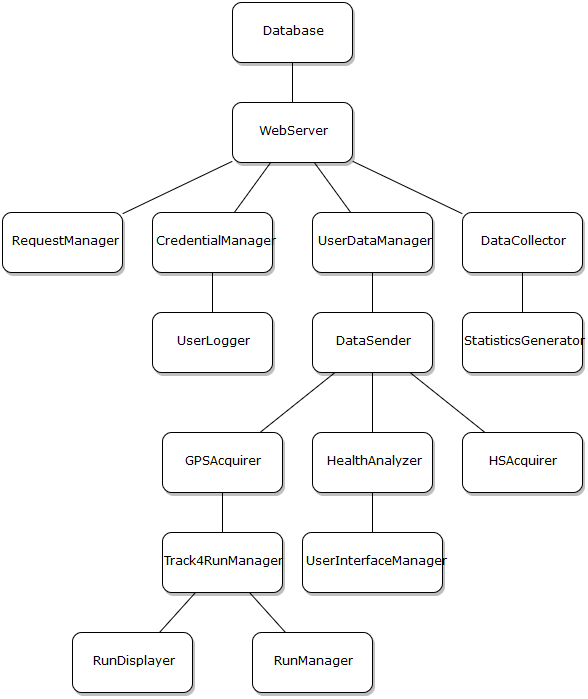
\includegraphics[scale=0.5]{Images/ImplementationPlan.png}
\caption{Implementation tree.}
\end{figure}

\noindent
The first component that will be developed is the Database due to the fact that almost every component of our system will exploit Database's features, also it's one of the most critical parts of the system, if it fails then all our system will as well, and lastly it forms the model of our system.
\medbreak
\noindent
The WebServer component will be developed right after the Database because it is also one of the most critical element of our system due to the fact that the third parties and the users will exploit this component to carry out every functionality that TrackMe offers.
\medbreak
\noindent
Then the components belonging to the third level of the tree will be developed since they form a big part of the business logic of our system and manage information requests.
\medbreak
\noindent
As soon as the DataSender is completed then the AutomatedSOS component will be developed, especially the HealthAnalyzer since, in order to have faster reaction time, it contains part of the logic of our system and also this component perform a critical functionality: calling an ambulance in case of need.
\medbreak
\noindent
Lastly the Track4RunManager will be developed followed by the 2 components of the Track4Run application.

\subsection{Integration and Test Plan}
Every component of the system must be subjected to Unit Testing during its development in order to identify as soon as possible any problem within the component. This way, before actually preceding to any Integration Test, we are pretty sure that all components work well in isolation.
\medbreak
\noindent
As said in the previous subsection the Integration Plan will also follow a Top-Down approach.

\subsection{System Testing}
Once the system is integrated completely and once it has an acceptable performance it will be tested as a whole. This due to the fact that in the future the system could possibly be subject to heavy workloads. System Testing will identify the following problems:

\begin{itemize}
\item Inefficient algorithms.
\item Query optimization problems: taking into account that the system's functionality heavily relies on queries this will for sure be a very useful test.
\item Hardware issues.
\item Network issues.
\end{itemize}

\noindent
More precisely two types of System Testing will be done:
\medbreak
\textbf{Load Testing ->} increasing the load of the system for a long period of time in order to find and solve memory leaks, buffer overflows, bad memory management and also identify upper limits of components.
\medbreak
\textbf{Stress Testing ->} trying to break the system by overwhelming its resources or by taking resources away from it will make sure that the system recovers gracefully after failure, this is very important for our system especially for AutomatedSOS components which are in charge of giving real time assistance to users that suffer from health issues.



